\chapter{Evaluation}
\label{ch:eval}


\section{Comparison with \porthos[1]}
\label{ch:eval:show}

\subsection{Compilation and unrolling}
\label{ch:eval:show:compil}

%As an example of the compilation and unrolling processes, consider the simple
%As a simple example of the compilation process discussed in Section~\ref{ch:impl:proc:x-compiler:compilation}, 
Consider two equivalent functions in C (left) and the \porthos[1] input language (right) represented in Figure~\ref{ex:test-both-cf}. %(in the C language on the left-hand side, the \porthos[1] input language on the right-hand side).
%The functions are state-equivalent (represent the same state machine) and 
The functions does not compute any useful value, however they contain three nested \texttt{while}-loops and thus can serve as an illustration of the differences in the program compilation and unrolling between \porthos[1] and \porthos[2].
%contains several syntactic elements (such as prefix increment and loop-breaking statements), which are supported by \porthos[2] comparing to its predecessor.
%In the Figure, the control-flow subgraph \xgraph[CF] of the non-unrolled event-flow graph is presented on the right-hand side (

\begin{figure}[!h]
%\begin{minipage}{.53\textwidth}
\begin{subfigure}[b]{.53\textwidth}\centering
\begin{lstlisting}[language=Java,basicstyle=\ttfamily\small]

void t0(int &x) {
     int a = 1;
     int c = 1;
     while (a == 1) {
         int b = 1;
         while (b == 1) {
             while (c == 1) {
                 x = c;
             }
             x = b;
         }
     }
     x = a;
 }
 
 
\end{lstlisting}
\caption{An example in the C language}
\label{ex:both-cf:ptsC}
\end{subfigure}
%\begin{minipage}{.45\textwidth}
\begin{subfigure}[b]{.45\textwidth}\centering
\begin{lstlisting}[language=Java,basicstyle=\ttfamily\small]
{ x }
thread t0 {
     a <- 1;
     c <- 1;
     while (a == 1) {
         b <- 1;
         while (b == 1) {
             while (c == 1) {
                 x := c
             };
             x := b
         };
     };
     x := a
 }
\end{lstlisting}
\caption{An example in the \porthos[1] input language}
\label{ex:both-cf:pts1}
\end{subfigure}
\caption{Example: A demonstrative cyclic function}
\label{ex:test-both-cf}
\end{figure}

The functions are processed by \porthos[2] or modified version \porthos[1] that is able to print same \xgraph[CF] as the new tool (for that, the control-flow instructions \texttt{if-then-else}, \texttt{while} and \texttt{sequence} are expanded recursively and the head and the tails of each instruction are bind by the method processing its parent).
The graph generation is performed via the open-source library \texttt{Graphviz}~\cite{ellson2001graphviz}).
%Each event of the control-flow graph contains the unique number (generated by the \texttt{hashCode} method) in curly brackets below the value, which is necessary for correct displaying the graph.

The Figure~\ref{ex:test-both-pic} illustrates the data structure which the functions in Figure~\ref{ex:test-both-cf} are compiled to.
The left-hand side picture represents the non-unrolled \xgraph[CF] generated by \porthos[2], and the right-hand picture represents the AST generated by \porthos[1].

In both pictures, the writes are denoted with the left-directed arrow `\lstinline{<-}', and the functions \lstinline{load} and \lstinline{store} denote the type of the shared memory event.
The primary transitions that denote unconditional jumps or if-true-transitions are pictured with solid lines, and the alternative transitions that denote if-false-transitions are pictured with dotted lines.
The graphs contains a single source event and a single sink event represented by the grey triangles (actually, the graph produced by \porthos[1] does not have sink and source nodes, but they were added to the picture for demonstrative purposes).
For clarity, all branching events, that in current example serve as the conditional events of loops, are highlighed with light-grey colour.

\begin{figure}[!h]
%
\begin{subfigure}[t]{.49\textwidth}\centering
  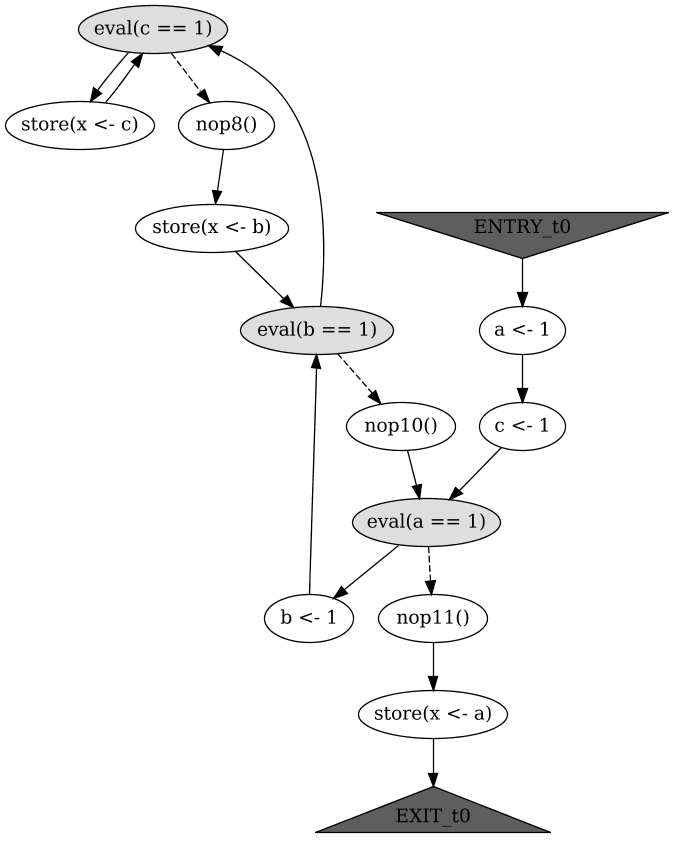
\includegraphics[width=\textwidth,keepaspectratio]{img/my/graphs/unrolling-comparison/PorthosC/t0.png}
  \hfill
  \caption{The compiled \xgraph{} of the function in Figure~\ref{ex:both-cf:ptsC}}
  \label{ex:both-cf:graph:ptsC}
\end{subfigure}
%
\begin{subfigure}[t]{.49\textwidth}\centering
  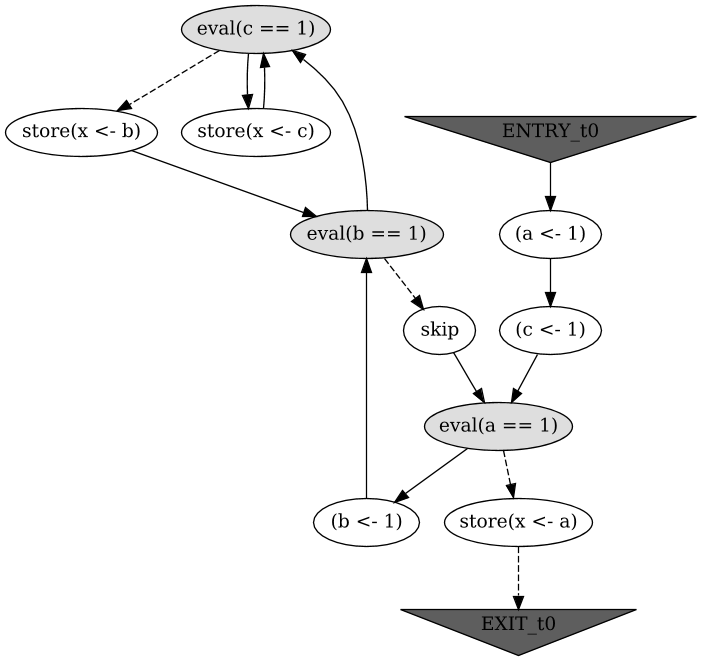
\includegraphics[width=\textwidth,keepaspectratio]{img/my/graphs/unrolling-comparison/Porthos/t0.png}
  \hfill
  \caption{The compiled AST of the function in Figure~\ref{ex:both-cf:pts1}}
  \label{ex:both-cf:graph:pts1}
\end{subfigure}
%
\caption{The control-flow graphs of the functions represented in Figure~\ref{ex:test-both-cf}}
\label{ex:test-both-pic}
\end{figure}

Two compiled the graphs are equivalent up to the extra \texttt{nop}-events in the \porthos[2] graph, that are necessary for correct encoding as it was discussed in Section~\ref{ch:enc:bmc:cf}, and \texttt{skip}-events in \porthos[1] graph.
However, the unrolled graphs presented in Figure~\ref{ex:test-both-pic-unroll} are different as \porthos[2] uses different unrolling algorithm.
The labels of events in the left-hand side picture (produced by \porthos[2]) are augmented by the unrolling depth number, which is separated from the event label by comma.

The unrolling algorithm used by \porthos[1] (right-hand side picture) unrolls \textit{all} loops $k$ times (where $k$ is the unrolling bound), and the unrolling algorithm of \porthos[2] unrolls loops so that not more than $k$ events are executed.
As it is illustrated by the picture, the new algorithm produces a better set of program executions (for example, the unrolled graph of \porthos[1] does not contain executions of the inner loops more than $k=2$ times, which makes the old unrolling algorithm not complete).
As the new unrolling algorithm uses the Deep-First Search, it discovers \textit{all} possible paths, therefore the result graph contains \textit{all} possible executions and thus is complete.

Note that the unrolled graph produced by \porthos[2] does not necessarily become a tree after removing the sink node.
Some branches of the graph are merged when the executions have the same event with the same unrolling depth number.
For example, primary transitions of both events `\lstinline{[b <- 1, 8]}' and `\lstinline{[store(x <- b), 8]}' (produced by executions of the first iteration of the \texttt{while} loop) lead to the same event `\lstinline{[eval(b == 1), 9]}' (the first event of the second iteration of the second loop).

\begin{figure}[!h]
%
\begin{subfigure}[b]{.6\textwidth}\centering
  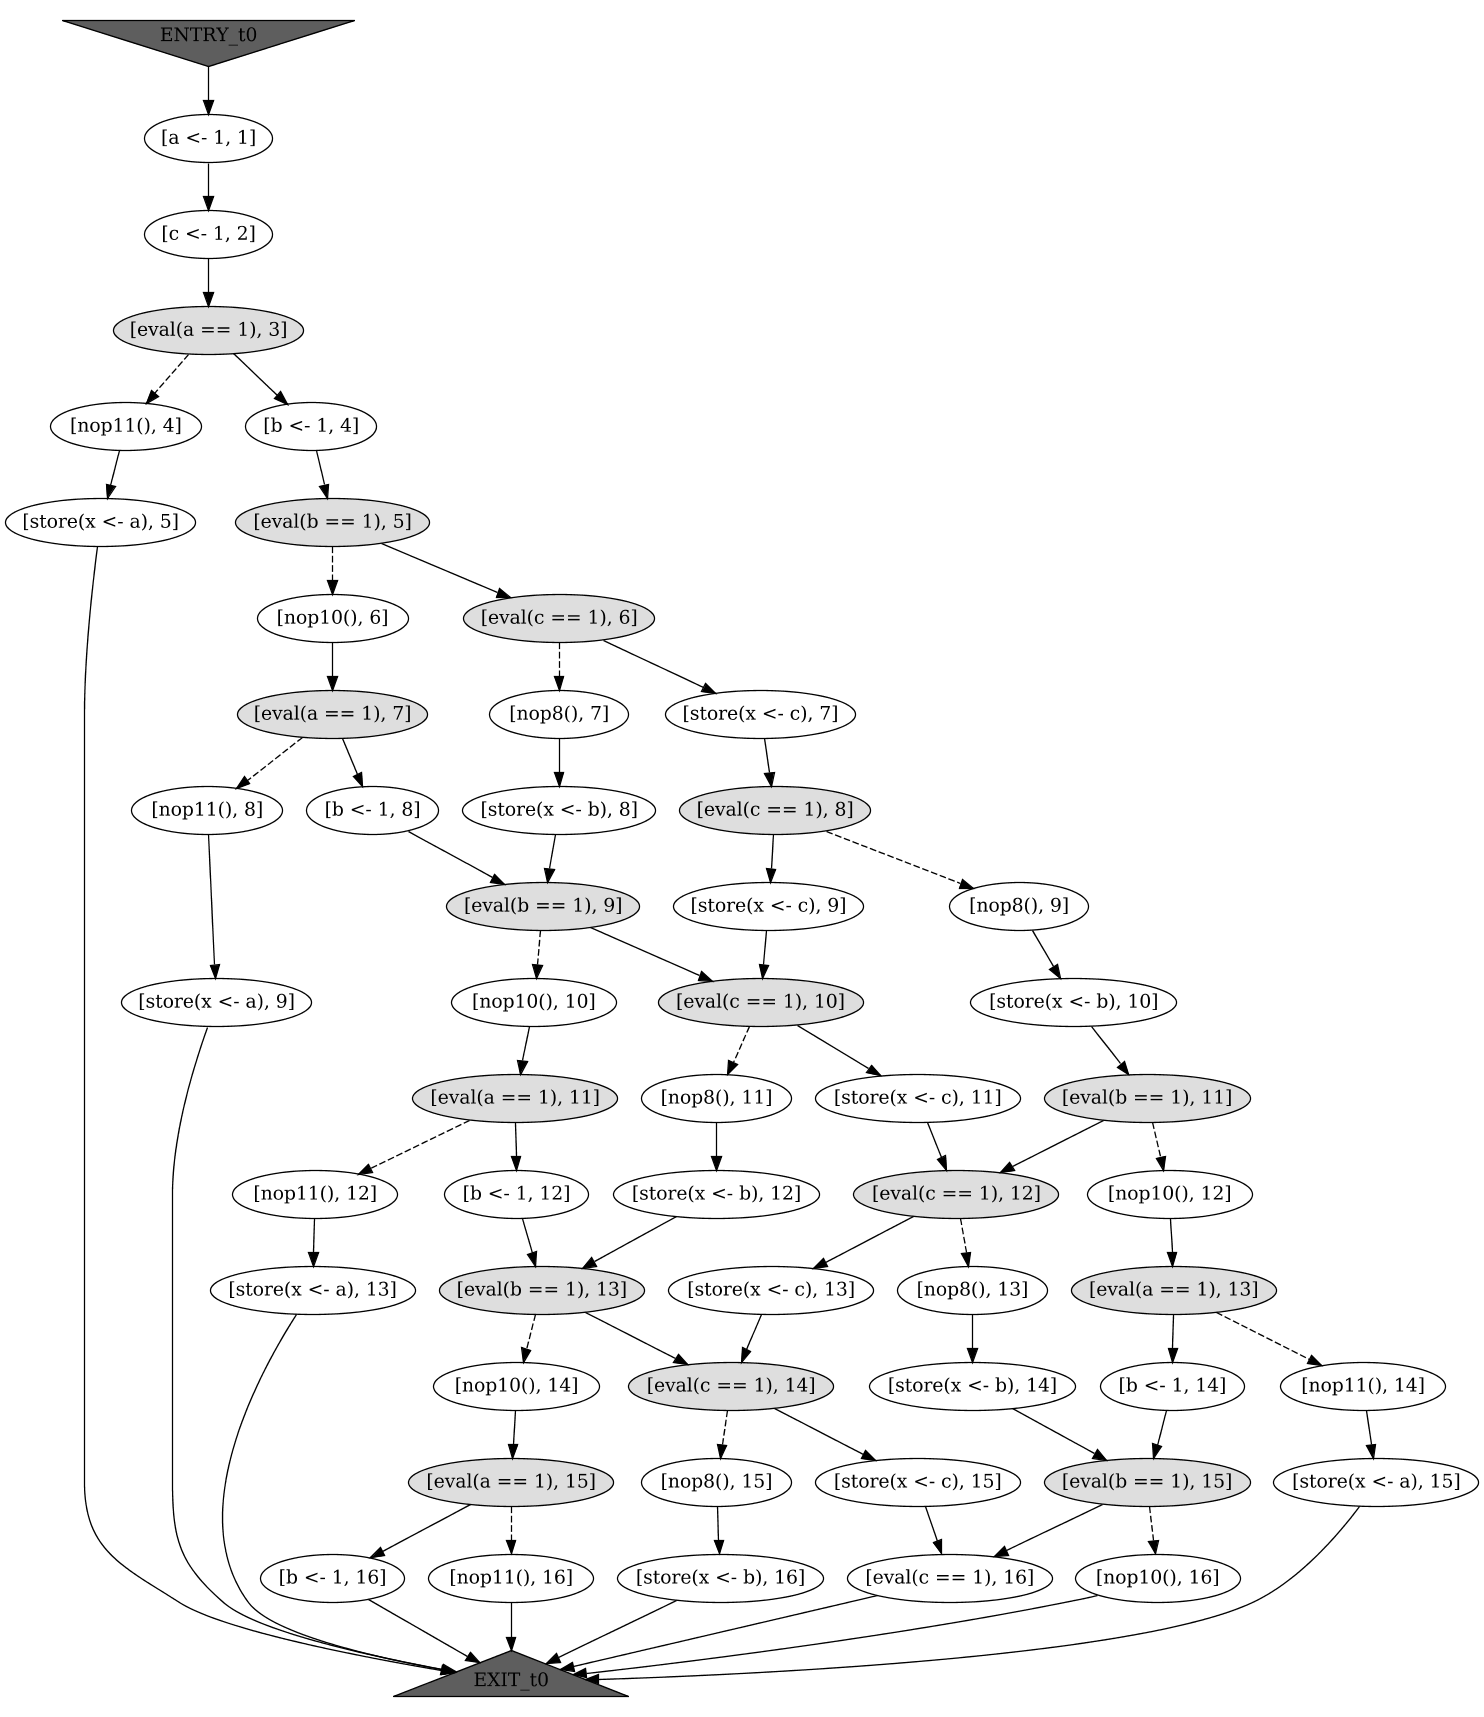
\includegraphics[height=.6\textheight,width=\textwidth]{img/my/graphs/unrolling-comparison/PorthosC/t0_unrolled.png}
  \hfill
  \caption{The unrolled \xgraph{} of the function in Figure~\ref{ex:both-cf:ptsC}}
  \label{ex:both-cf:graphU:ptsC}
\end{subfigure}
\hfill
%
\begin{subfigure}[b]{.3\textwidth}\centering
  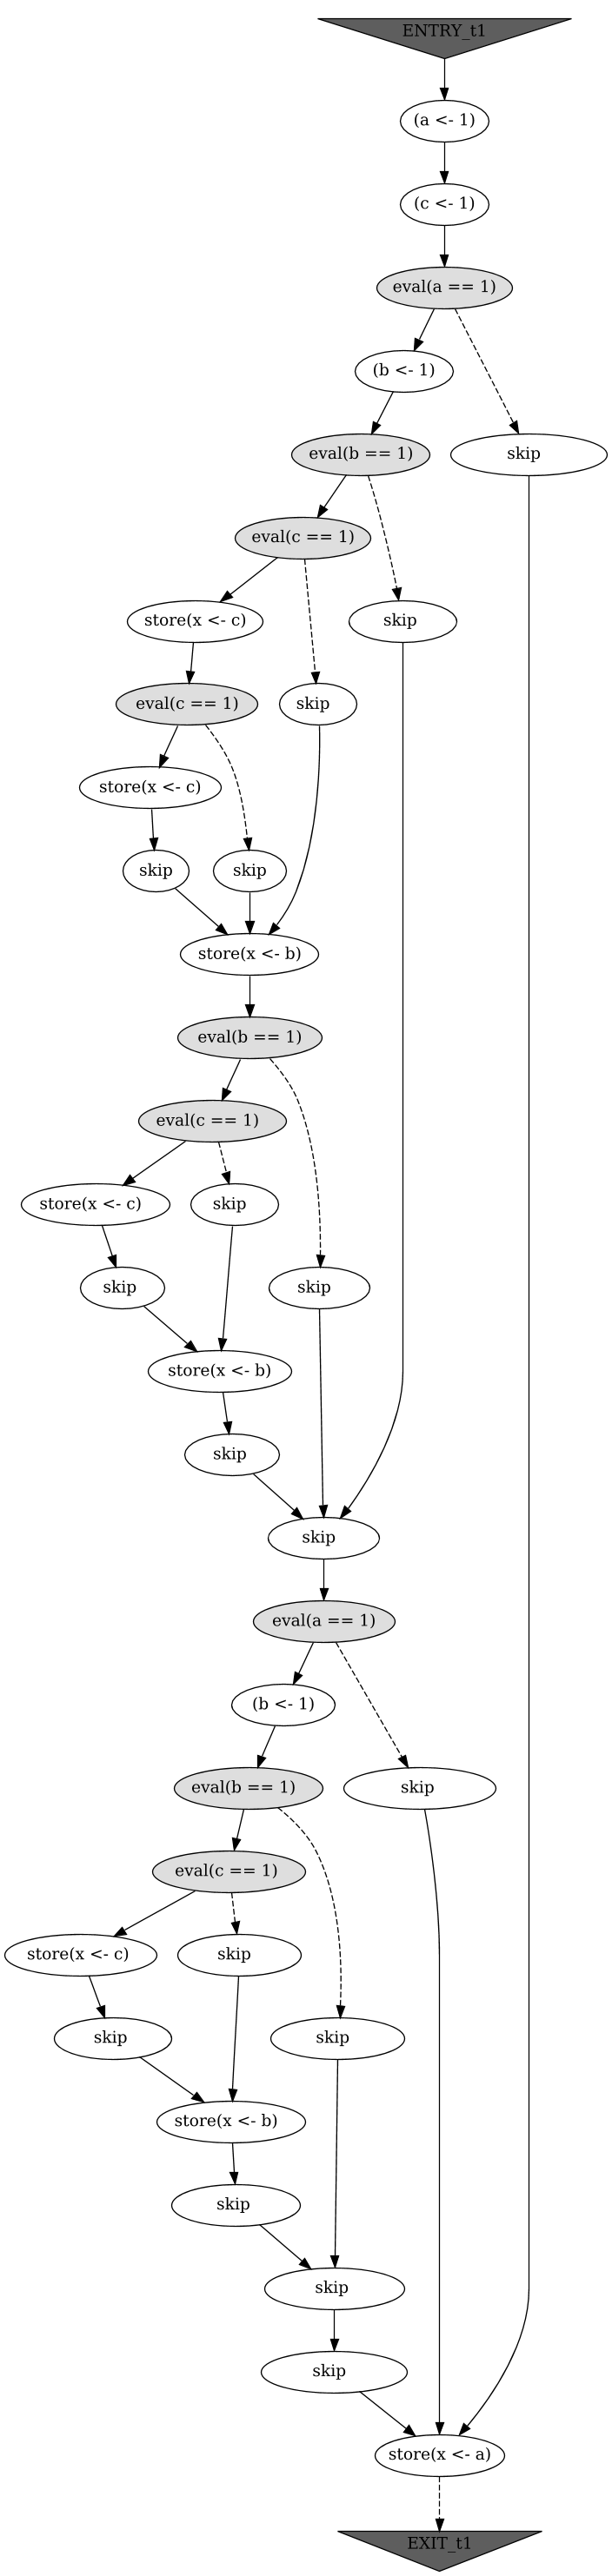
\includegraphics[height=.9\textheight,width=\textwidth]{img/my/graphs/unrolling-comparison/Porthos/t0_unrolled.png}
    \caption{The unrolled AST of the function in Figure~\ref{ex:both-cf:pts1}}
    \hfill
  \label{ex:both-cf:graphU:pts1}
\end{subfigure}
\hfill
%
\caption{The unrolled control-flow graphs of the functions represented in Figure~\ref{ex:test-both-cf}}
\label{ex:test-both-pic-unroll}
\end{figure}

%The arguments \lstinline{x} and \lstinline{y} of the function are passed by reference, therefore they are treated as global variables.
%The local variable declaration `\lstinline{int r;}' produces no events (it is processed by the X-graph pre-compiler that invokes the memory manager to create the new local variable \lstinline{r}).
%The first event `\lstinline{load(reg_tmp0 <- x}' loads the value of the global variable \lstinline{x} into the temp register \lstinline{reg_tmp0} in order to satisfy the requirement that all computation must be performed over local variables;
%note that each element of the computational tree `\lstinline{eval(eval(eval(5 + eval(eval(4 / 2) * reg_tmp0)) % 3) == 1)}' is represented by a local memory unit (either \texttt{XComputationEvent} or \texttt{XConstant} or \texttt{XRegister}).
%The node of this computational event in the control-flow graph has two outgoing edges, the primary edge to the `\lstinline{load(reg_tmp1 <- y}', the first event of the then-branch of the while-loop, and the alternative edge to the \lstinline{nop}-event representing the only event of the else-branch.

%As is was discussed in Section~\ref{ch:impl:model:xgraph}, all computation events have no impact to the global state of the concurrent system.
%Therefore, the interpreter does not \textit{emit} computational events, but it \textit{creates} them.
%This means, when the \texttt{Y2XConverterVisitor} processes the expression tree `\lstinline{(5 + 4/2 * x) 3 == 1}', it calls the method \texttt{createComputationEvent} of the interpreter that only creates the computation event and does not change its state.
%However, once the converter meets the global variable \lstinline{x}, it calls the interpreter method \texttt{emitMemoryEvent} to copy its value to a temp register; since it meets the global variables involved to the computation before it ends to process the whole computation expression, the values of all these global variables will be copied to temp registers \textit{before} the computation expression is used by any other event.
%Note that if the computation expression has not been used by any other event (for example, as the constant \lstinline{1} in the following C code: `\lstinline{foo(); 1; bar();}'), it is lost from the model (by the term \textit{use} here we mean that the computation event is evaluated as a guard or assigned to another memory unit).


%\subsection{The X-graph unrolling}
%\label{ch:eval:show:unrol}

%Once the \xgraph[CF] is constructed, it should be unrolled to an acyclic flow-graph (as it was discussed in Section~\ref{ch:impl:proc:x-unroll}).
%The Figure~\ref{ex:unrolling} shows the control-flow subgraph \xgraphU[CF] of the event-flow graph from the previous example (see Figure~\ref{ex:compilation}) unrolled up to bound $k=16$.
%


%TODO: here (or better in Chap 5 ) say about 'we tried different encoding schemes !!!!!!!!!!!!!!!!!!!!!!!!!!!!!!!!!!!!!!!!!!!!!!!!!!!!!!!!!!!!!!!!!!!!!!!!!!!
 
%Also note that comparing to the unrolling bound description given in Section~\ref{ch:impl:proc:x-unroll}, 
%As the distinction between complete and incomplete sink nodes is not implemented yet, 

%\begin{figure}[!h]
%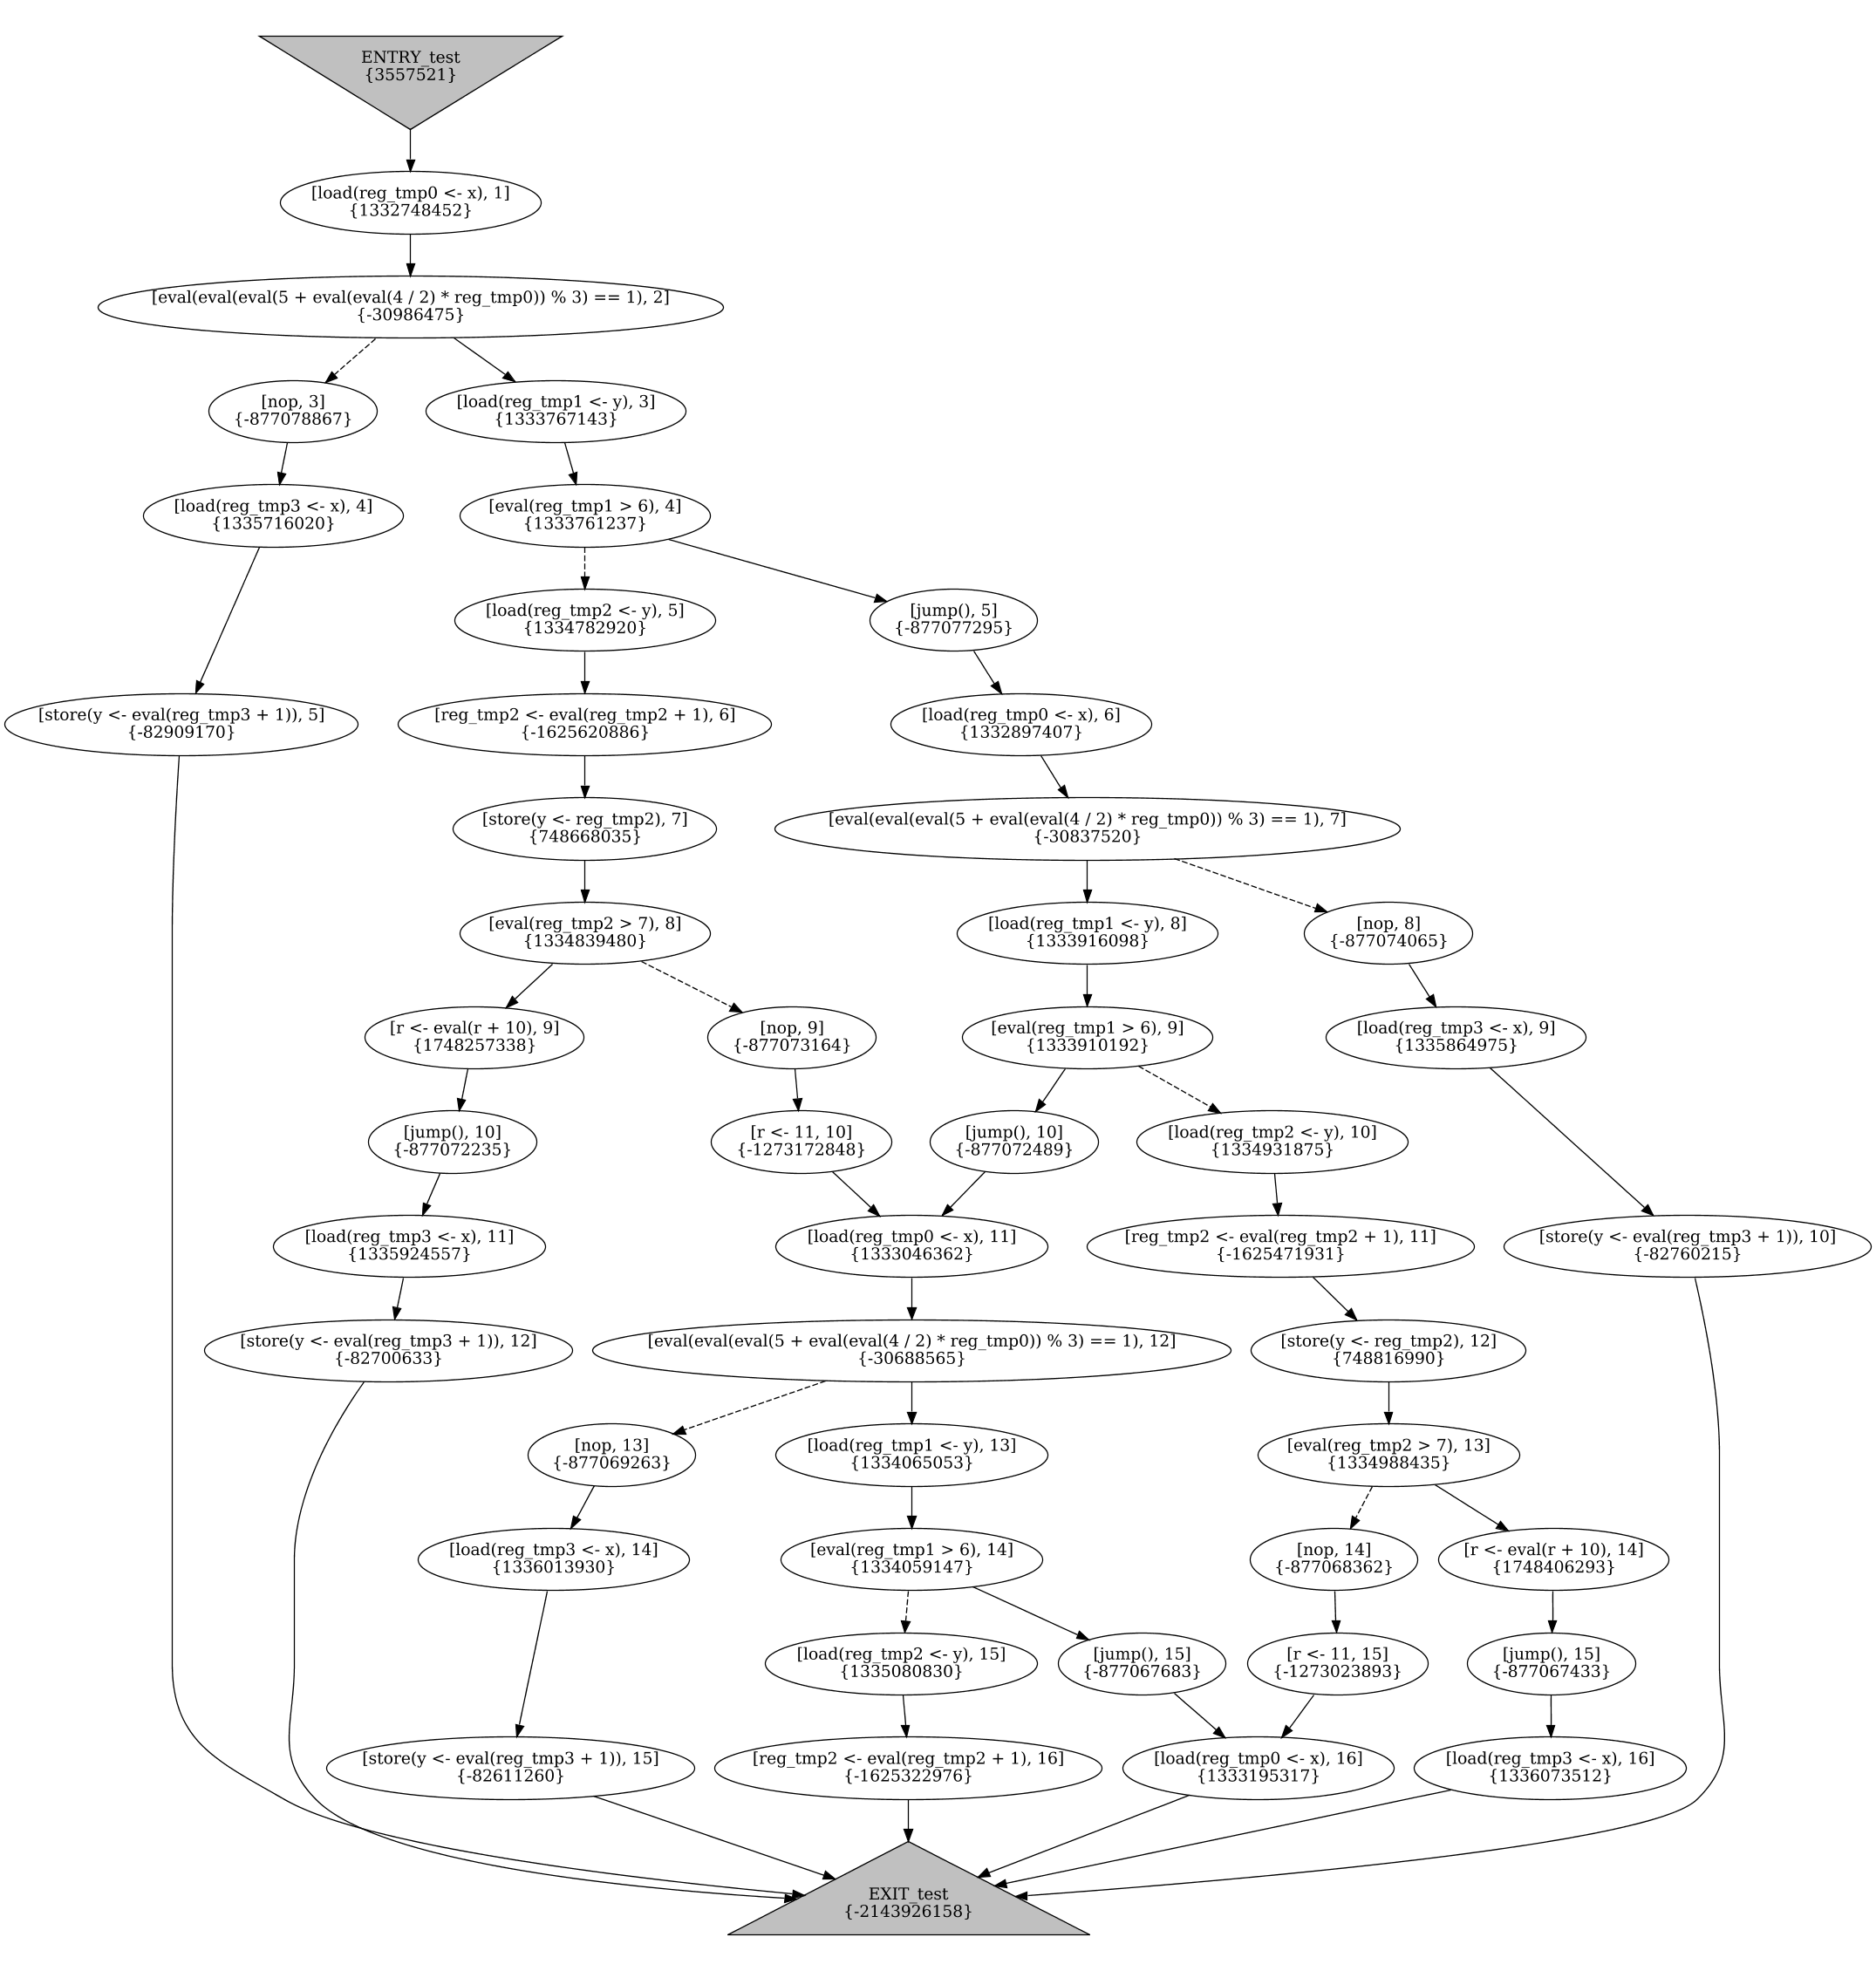
\includegraphics[width=\textwidth,height=\textheight]{img/my/graphs/test_unrolled.png}
%\caption{Unrolling of the event-flow graph presented in Figure~\ref{ex:compilation}}
%\label{ex:unrolling}
%\end{figure}


\section{Performance evaluation}
\label{ch:eval:perf}

As an example of the C program liable for the reachability and portability analysis, consider the Dekker's algorithm for mutual exclusion of two processes, originally described by Dijkstra~\cite{dijkstra1962over}; the program is presented in Appendix~\ref{apx:dekker}.
For testing \porthos[1], we used the same file in old \porthos{} input language (\texttt{dekker.pts}), which was used in evaluation tests in the original paper~\cite{Porthos17a}.

\subsection{State reachability analysis}
\label{ch:eval:perf:reach}

%For checking reachability of the final states of the unrolled graphs compiled for a certain hardware architecture, the tool encodes both program and hardware memory model constraints as it was discussed in Section~\ref{ch:enc:bmc}.
%The result formula is then solved by the Z3 

%TO-DO: fix interface
%To run \porthos[2] in reachability analysis mode, we use the command `\lstinline{mousq

%\textbf{TODOOOOOOOOOOOOOOOOOOOOO!!!! Re-compute tests with new counting of encoding}
When running in the state reachability analysis mode, \porthos[2] produces the following output:

\begin{lstlisting}
$ java PorthosC --reachability --input benchmarks/C11/Dekker.c \
      --bound 27 --target TSO
0.288: Interpretation...
0.426: Unrolling...
0.533: Program encoding...
0.701: Program domain encoding...
#=193 (107)
34.187: Memory model encoding...
36.818: Solving...
{
  "result": "NonReachable",
  "mainTimer": {
    "elapsedTimeSec": 36.163
  },
  "timers": {
    "Interpretation": {
      "elapsedTimeSec": 0.132
    },
    "ProgramDomainEncoding": {
      "elapsedTimeSec": 32.486
    },
    "Solving": {
      "elapsedTimeSec": 0.345
    },
    "Unrolling": {
      "elapsedTimeSec": 0.061
    },
    "MemoryModelEncoding": {
      "elapsedTimeSec": 2.631
    },
    "ProgramEncoding": {
      "elapsedTimeSec": 0.168
    }
  },
  "errors": []
}
\end{lstlisting}

For time benchmarking we ran the tool $5$ times and computed the median of the encoding time.
Benchmarking was performed on the Linux machine 8-core Intel(R) Core(TM) i7-3632QM CPU @ 2.20GHz, Java(TM) SE Runtime Environment (build 1.8.0\_161-b12) (Java virtual machine was configured by default parameters).
The time was measured by the tool itself via the native Java method \texttt{System.currentTimeMillis}.

%For \porthos[1] we specify the unrolling bound $k_1 = 2$, and for \porthos[2] the bound is $k_2 = 21$ ().
As the unrolling algorithm has been changed, the number of events after unrolling differs considerably.
Therefore, the correct performance comparison with \porthos[1] is not manageable as the performance of the tools depends directly on number of events.
For example, with the bound $k_1=2$ \porthos[1] produces $59$ events (among them, $51$ shared-memory events) with the program domain encoding time 4.608 sec,
and with the bound $k_1=3$ \porthos[1] produces $95$ events (among them, $107$ shared-memory events) with the program domain encoding time 21.475 sec;
whereas \porthos[2] with the bound $k_2=17$ produces $57$ ($31$) events with the program domain encoding time 1.734, and with the bound $k_2=27$ it produces $193$ events (among them, $107$ shared-memory events, which equal to the number of shared-memory events produced by \porthos[1] with the bound $k_1=3$) with the time 32.673 sec.
Therefore, the new unrolling scheme has made the analysis complete but at the same time it reduced the performance considerably.
%The last result shows that with the bounds $k_1=3$ and $k_2=27$ both tools have executed same number of loops  almost equivalent as they
%However, the program domain encoding and memory model encoding schemes have not been changed considerably comparing to \porthos[1], therefore the execution time 
%Although, the performance depends directly on number of events, 

%\porthos[2] shows the full encoding time for the Dekker's algorithm 2.699 sec (from which 0.152 sec spent for the program encoding, and other part spent for the memory model encoding).
%In contrast, \porthos[1] shows the encoding time 6.152 sec (from which 0.223 sec spent for the program encoding). %, which is considerably better result.
%Thus, the performance of the encoding stage has been\textbf{ improved in 2.7 times}.

Note, that the time spent by \porthos[2] for the interpretation and unrolling stages remains to be negligible comparing to the full encoding time.
Therefore, we conclude that the new architecture implies no performance overhead comparing to the previous version of the tool.
The time spent by the SMT solver while considering the SMT formula encoded by \porthos[2] was 0.039 sec, and in case of \porthos[1] the time was 1.291 sec.
The number of events in the event-flow graph of \porthos[2] is 82 events (among them 59 memory events), and the number of events encoded by \porthos[1] is 95 (among them 51 memory events).
Even though the number of memory events processed by \porthos[1] was less, the time of solving the result SMT-formula was significantly more.

<TODO: above as table>

%We consider this improvement to be the result of some technical optimisations applied to the encoding stage of \porthos[2].
%The major optimisation is the \textit{memoisation} of frequently requested calls.
%For example, the code of \porthos[1] contains 39 calls that take the subset of a set of events, 10 of them are performed in a loop over all events (in \texttt{Domain.encode} method of \porthos[2]).
%The pattern is the following: `\lstinline{program.getEvents().stream().filter(e -> e instanceof MemEvent || e instanceof Local).collect(Collectors.toSet())}'.
%%TODO: refactor X-program inheritance
%In \porthos[2], these calls were replaced by the lazily initialisable memoisation methods (see \texttt{XProgram}): \\
%
%\vspace{-1em}
%\begin{lstlisting}[language=Java]
%public ImmutableSet<XMemoryEvent> getMemoryEvents() {
%    return memoryEvents != null
%        ? memoryEvents
%        : (memoryEvents = getAllNodesExceptSource(XMemoryEvent.class));
%}
%\end{lstlisting}

%TODO: say how much the \textit{immutable data structures} helped (as it was discussed in Chapter~\ref{ch:impl}).

%<TODO: compare numbers of clauses of SMT formulas>

<TODO: profile both programs, say sth about memory usage!> 


\subsection{Portability analysis}
\label{ch:eval:perf:port}

For evaluating the tool working in the portability analysis mode, we used the same file \texttt{Dekker.c} tested for the state-portability from TSO to SC: %TODO: Say sth about state-portability

%!!! \textit{\textbf{TODO: change the main class name to PorthosC }} !!!

\begin{lstlisting}
$ java PorthosC --portability --input benchmarks/C11/Dekker.c \
      --bound 27 --source TSO --target SC --state
0.359: Interpretation...
0.364: Unrolling...
0.590: Unrolling...
0.623: Program encoding...
0.847: Program domain encoding...
#=193 (107)
#=193 (107)
66.541: Memory model encoding...
72.321: Solving...
{
  "result": "StatePortable",
  "iterations": 0,
  "mainTimer": {
    "elapsedTimeSec": 73.02
  },
  "timers": {
    "ProgramEncoding": {
      "elapsedTimeSec": 0.223
    },
    "MemoryModelEncoding": {
      "elapsedTimeSec": 5.779
    },
    "Interpretation": {
      "elapsedTimeSec": 0.248
    },
    "Solving": {
      "elapsedTimeSec": 0.699
    },
    "ProgramDomainEncoding": {
      "elapsedTimeSec": 65.693
    },
    "Unrolling": {
      "elapsedTimeSec": 0.022
    }
  },
  "errors": []
}
\end{lstlisting}

As the portability analysis requires compiling the program under two memory models, the overall program domain encoding time 65.693 sec is almost double as the same time in reachability analysis mode (\porthos[1] shows program domain encoding time 41.027 sec with the bound $k_1=3$).


\subsection{New features}
\label{ch:eval:perf:feat}

%The revised design of \porthos{} tool includes the following new features:
Apart from redesigning the tool architecture and extending the input language, we added support for basic constructions used in \textit{Kernel litmus tests}~\cite{alglave2018frightening}.
Although, current version of \porthos[2] only supports some basic macros of the Linux kernel (such as \texttt{READ\_ONCE} and \texttt{WRITE\_ONCE} for atomic load and store with relaxed memory ordering) as the support for kernel-specific memory barriers goes out of the scope of current thesis.
Note that, comparing to the \porthos[1], adding support for new functions in \porthos[2] does not require changing the input language grammar, this is carried by invocation hooking mechanism described in Section~\ref{ch:impl:proc:x-compiler:hooking}.

As an example, consider the SB litmus test for the Linux kernel (which is similar to the one presented in Figure~\ref{simple_wmm_x86}):
\begin{lstlisting}
{ int x = 0; int y = 0;}

P0(volatile int* y, volatile int* x) {
  int r0;
  WRITE_ONCE(*x,1);
  r0 = READ_ONCE(*y);
}

P1(volatile int* y, volatile int* x) {
  int r0;
  WRITE_ONCE(*y,1);
  r0 = READ_ONCE(*x);
}

exists(x == 0 && y == 0)
\end{lstlisting}

If verifying this litmus test by \porthos[2] in the state reachability mode, the test passes for TSO memory model and fails for SC model.

